\documentclass[tikz,border=5pt]{standalone}
\usepackage{pgfplots}
\pgfplotsset{compat=1.18}
\definecolor{curveblue}{RGB}{61,94,115}
\begin{document}
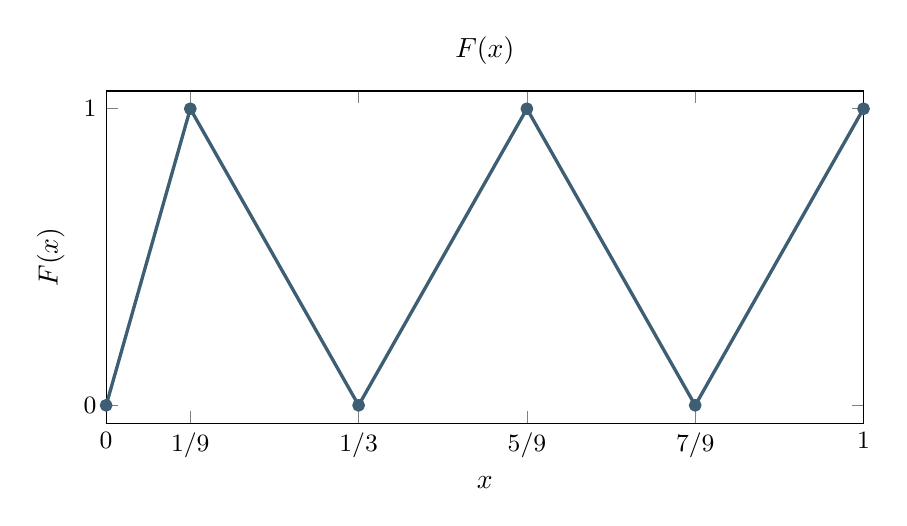
\begin{tikzpicture}
% Four hidden ReLU units; five exact affine full-range pieces on [0,1].
\begin{axis}[width=11.2cm,height=5.8cm,xmin=0,xmax=1,ymin=-0.06,ymax=1.06,xlabel={$x$},ylabel={$F(x)$},xtick={0,0.111111111111,0.333333333333,0.555555555556,0.777777777778,1},xticklabels={$0$,$1/9$,$1/3$,$5/9$,$7/9$,$1$},ytick={0,1},title={$F(x)$},tick label style={font=\small}]
\addplot[curveblue,very thick,line join=round,line cap=round,mark=*,mark size=1.7pt] coordinates {(0,0) (0.111111111111,1) (0.333333333333,0) (0.555555555556,1) (0.777777777778,0) (1,1)};
\end{axis}
\end{tikzpicture}
\end{document}
